%%%%%%%%%%%%%%%%%%%%%%%%%%%%%%%%%%%%%%%%%%%%%%%%%%%%%%%%%%%%%%%%%%%%%%%%%
\section{Proofs}  %%%%%%%%%%%%%%%%%%%%%%%%%%%%%%%%%%%%%%%%%%%%%%%%%%%%%%%
\label{rs:sec:proofs}

Section~\ref{rs:sec:pflemmas} contains the proofs of Lemmas~\ref{rs:lem:samplecomp} and~\ref{rs:lem:dispbound}.
Section~\ref{rs:sec:pfqdisp} presents the proof for our results on the displacement of the output of a single call to Quicksort (Theorem~\ref{rs:thm:quickdisp}), and Section~\ref{rs:sec:pfmdisp} shows our result on the displacement of the Copeland aggregation of multiple outputs (Theorem~\ref{rs:thm:multidisp}).

%%%%%%%%%%%%%%%%%%%%%%%%%%%%%%%%%%%%%%%%%%%%%%%%%%%%%%%%%%%%%%%%%%%%%%%%%
\subsection{Lemmas~\ref{rs:lem:samplecomp} and~\ref{rs:lem:dispbound}}
\label{rs:sec:pflemmas}

We start by briefly presenting a result from graph theory that will be useful in the proof of Lemma~\ref{rs:lem:samplecomp}.
A \emph{tournament} is a directed graph obtained by assigning a direction to every edge of a complete graph.
The \emph{score sequence} of a tournament is defined as the nondecreasing sequence of the vertices' outdegrees.
The following proposition is by \citet{landau1953dominance}.

\begin{proposition}
\label{rs:prop:landau}
Let $(s_1, \ldots, s_N)$ with $0 \le s_1 \le \cdots \le s_N$ be the score sequence of a tournament on $N$ vertices.
Then,
\begin{align*}
\frac{n - 1}{2} \le s_n \le \frac{N + n - 2}{2} \quad \forall\ n \in [N].
\end{align*}
\end{proposition}

We use a tournament on $N$ vertices to represent the outcome of a comparison between each pair of items.
In particular, we represent the outcome $i \prec j$ by an edge $(i, j)$.
In this case, the outdegree of a vertex $i$ corresponds to the number of items which ``won'' in a comparison against $i$.
Note that the comparison outcomes do not need to be transitive, i.e., the tournament can contain cycles.

The proof of Lemma~\ref{rs:lem:samplecomp} is adapted from standard results on Quicksort, see, e.g., \citet[][Section 3.3.3]{dubhashi2009concentration}.
These results are based on the fact that it is likely that the random choice of pivot leads to a well-balanced partition into subsets $\mathcal{L}$ and $\mathcal{R}$.
In our setting, the comparison outcomes do not need to be consistent with an ordering of the items, therefore we cannot use the standard argument based on the pivot's \emph{rank}.
Instead, we use the tournament representation of the comparison outcomes and analyze the pivot's \emph{out-degree} (using Proposition~\ref{rs:prop:landau}) to ensure that the partition is balanced often enough.

\begin{proof}[Proof of Lemma~\ref{rs:lem:samplecomp}]
We show that the maximum call depth of Quicksort is at most $\Ceil{48 \log N}$ with high probability.
The statement follows by noting that at most $N$ comparisons are used at each level of the call tree.

By Lemma~\ref{rs:lem:termination}, Quicksort samples a comparison outcome for each pair of items at most once.
Therefore, we can represent these (a priori unobserved) pairwise outcomes as a tournament $\mathcal{T} = ([N], \mathcal{A})$.
At each step of the recursion, we select a pivot $p$ uniformly at random in the set $\mathcal{V}$ (line~\ref{rs:line:pivot}), and compare it to the rest of the items in the set (line~\ref{rs:line:comp}).
Let $\mathcal{T}_{\mathcal{V}}$ denote the subgraph of $\mathcal{T}$ induced by $\mathcal{V}$.
Given that the comparison outcomes follow from the edges of the tournament, $\mathcal{L}$ is equal to the set of incoming neighbors of $p$ in $\mathcal{T}_{\mathcal{V}}$.
(Correspondingly, $\mathcal{R}$ is equal to the set of the outgoing neighbors.)
Hence, the outdegree of $p$ in $\mathcal{T}_\mathcal{V}$ determines how balanced the partition is.
The probability that the outdegree of $p$ lies in the middle half of the score sequence is $1/2$, and if it does, Proposition~\ref{rs:prop:landau} tells us that
\begin{align*}
\frac{\Abs{\mathcal{V}} - 7}{8} \le \mathrm{outdeg}(p) \le \frac{7 \Abs{\mathcal{V}} - 5}{8}.
\end{align*}
In this case, at the end of the partition $\Abs{\mathcal{L}}$ and $\Abs{\mathcal{R}}$ are of size at most $7\Abs{\mathcal{V}}/8$, and in at most $\log_{8/7}(N) \le 8 \log N $ such partitions we get to a subset of size one and match the terminating case.
Even though we do not select, every time, the pivot in the middle half, it is unlikely that more than $c \cdot 8 \log N$ recursions are needed (for some small constant $c$) to select the pivot in the middle range at least $8 \log N$ times.
Let $z_d$ i.i.d $\sim \text{Bern}(1/2)$ be the indicator variable for the event ``the pivot is selected in the middle half at level of recursion $d$''.
Using a Chernoff bound, we have
\begin{align*}
\Prob{\sum_{d=1}^{\Ceil{48 \log N}} z_d \le 8 \log N} \le \frac{1}{N^2},
\end{align*}
i.e., the depth of a leaf in the call tree is at most $\Ceil{48 \log N}$ with probability at least $1 - 1/N^2$.
As there are at most $N$ leaves in the tree, the \emph{maximum} depth is bounded by the same value with probability at least $1 - 1/N$.
\end{proof}

In order to prove Lemma~\ref{rs:lem:dispbound}, we introduce some additional notation.
Let $\mathbf{S}_N$ be the set of all permutations on $[N]$.
For any $\sigma \in \mathbf{S}_N$ and $\mathcal{V} \subseteq [N]$, let $\sigma_{\mathcal{V}} : \mathcal{V} \to \{1, \ldots, \Abs{\mathcal{V}}\}$ be the ordering induced by $\sigma$ on $\mathcal{V}$.
We generalize the definition of displacement as
\begin{align*}
\Disp[\mathcal{V}]{\sigma, \tau} = \sum_{i \in \mathcal{V}} \Abs{\sigma_{\mathcal{V}}(i) - \tau_{\mathcal{V}}(i)}.
\end{align*}
For conciseness, we use the shorthand $\Disp[\mathcal{V}]{\sigma} \doteq \Disp[\mathcal{V}]{\sigma, \Id}$, where $\Id$ is the identity permutation.

\begin{proof}[Proof of Lemma~\ref{rs:lem:dispbound}]
Denote by $\mathcal{A}$ the collection of working sets that were used as input to one of the recursive calls to Quicksort.
For $\mathcal{V} \in \mathcal{A}$, let $\mathcal{E}_{\mathcal{V}}$ be the set of pairs sampled by Quicksort to partition $\mathcal{V}$ and which result in an error.
Note that $\mathcal{E}_{\mathcal{V}} \cap \mathcal{E}_{\mathcal{V}'} = \varnothing$ for $\mathcal{V} \ne \mathcal{V}'$, and that $\bigcup_{\mathcal{V}} \mathcal{E}_{\mathcal{V}} = \mathcal{E}$.
We will show that for all $\mathcal{V} \in \mathcal{A}$,
\begin{align}
\label{rs:eq:recursive}
\Disp[\mathcal{V}]{\sigma}
    \le \Disp[\mathcal{L}]{\sigma} + \Disp[\mathcal{R}]{\sigma}
    + 2 \sum_{\mathclap{(i, j) \in \mathcal{E}_{\mathcal{V}}}}\; \Abs{i - j},
\end{align}
where $\mathcal{L}, \mathcal{R} \in \mathcal{A}$ are the two sets obtained at the end of the partition operation.
The lemma follows by taking $\mathcal{V} = [N]$ and recursively bounding \Disp[\mathcal{L}]{\sigma} and \Disp[\mathcal{R}]{\sigma}.

Consider the partition operation on $\mathcal{V}$, with pivot $p$, resulting in partitions $\mathcal{L}$ and $\mathcal{R}$.
Let $\tilde{\sigma}$ be the ordering on $\mathcal{V}$ that
\begin{enuminline}
\item \label{rs:itm:tsa} ranks $\mathcal{L}$ at the bottom, $p$ in the middle and $\mathcal{R}$ at the top, and
\item \label{rs:itm:tsb} matches the identity permutation on $\mathcal{L}$ and $\mathcal{R}$, i.e., $\Disp[\mathcal{L}]{\tilde{\sigma}} = \Disp[\mathcal{R}]{\tilde{\sigma}} = 0$.
\end{enuminline}
In a sense, $\tilde{\sigma}$ is the ordering that would be obtained if there were no further errors in the remaining recursive calls.
Using the triangle inequality, we have that
\begin{align}
\label{rs:eq:tridisp}
\Disp[\mathcal{V}]{\sigma} \le \Disp[\mathcal{V}]{\sigma, \tilde{\sigma}} + \Disp[\mathcal{V}]{\tilde{\sigma}}.
\end{align}
By definition of $\tilde{\sigma}$, we have that
\begin{align}
\label{rs:eq:recdisp}
\Disp[\mathcal{V}]{\sigma, \tilde{\sigma}}
    = \Disp[\mathcal{L}]{\sigma, \tilde{\sigma}} + \Disp[\mathcal{R}]{\sigma, \tilde{\sigma}}
    = \Disp[\mathcal{L}]{\sigma} + \Disp[\mathcal{R}]{\sigma},
\end{align}
where the first equality follows from \ref{rs:itm:tsa}, and the second follows from \ref{rs:itm:tsb}.

\begin{figure}[t]
\centering
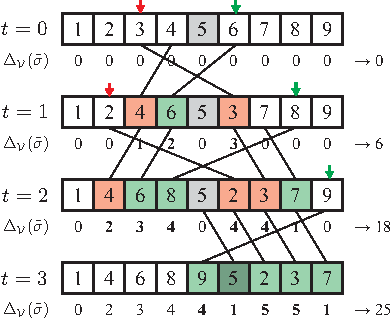
\includegraphics[scale=1.2]{rs-qsort}
\caption{Illustration of the decomposition of \Disp[\mathcal{V}]{\tilde{\sigma}} into contributions of individual errors over a sequence of steps.
In this example, $\mathcal{V} = \{ 1, \ldots, 9 \}$, $p = 5$ and there are five errors.
At step $t = 1$, we process the errors $(5, 3)$ and $(5, 6)$;
at step $t = 2$, we process the errors $(5, 2)$ and $(5, 8)$, and finally, at step $t = 3$, we process the error $(5, 9)$.
The shifts caused by an error are highlighted in red and green.
In this example, $\Disp[\mathcal{V}]{\tilde{\sigma}} = 25 < 2 \sum_{(i,j) \in \mathcal{E}_{\mathcal{V}}} \Abs{i - j} = 26$.
}
\label{rs:fig:qsort}
\end{figure}

Finally, we bound $\Disp[\mathcal{V}]{\tilde{\sigma}}$.
Let $\mathcal{E}_{\mathcal{V}}^- = \{ (p, i) \in \mathcal{E}_{\mathcal{V}} : i < p \}$, and similarly $\mathcal{E}_{\mathcal{V}}^+ = \{ (p, i) \in \mathcal{E}_{\mathcal{V}} : i > p \}$.
Without loss of generality, we can assume that $\mathcal{V}$ consists of consecutive integers, and that $\kappa \doteq \Abs{\mathcal{E}_{\mathcal{V}}^-} \le \Abs{\mathcal{E}_{\mathcal{V}}^+}$.
We proceed as follows: starting from the ranking $\Id_{\mathcal{V}}$, we progressively incorporate errors into the ranking, ending with $\tilde{\sigma}$ once all errors have been treated.
To understand the effect of each error on \Disp[\mathcal{V}]{\tilde{\sigma}}, we look at errors in the following specific sequence.
\begin{enumerate}
\item At steps $t = 1, \ldots, \kappa$, we consider the $t$-th ``smallest'' errors in $\mathcal{E}_{\mathcal{V}}^-$ and $\mathcal{E}_{\mathcal{V}}^+$.
That is, we process $(p, i) \in \mathcal{E}_{\mathcal{V}}^-$ and $(p, i') \in \mathcal{E}_{\mathcal{V}}^+$ such that $\Abs{p - i}$ and $\Abs{p - i'}$, respectively, are the smallest among errors not yet treated.

\item At steps $t = \kappa + 1, \ldots, \Abs{\mathcal{E}_{\mathcal{V}}^+}$, we process the remaining errors in $\mathcal{E}_{\mathcal{V}}^+$, once again in increasing order of distance to  $p$.
\end{enumerate}
Figure~\ref{rs:fig:qsort} illustrates the state of the ranking at different steps on a concrete example.
We start with the first case, i.e., $t \le \kappa$.
The effect of the errors $(p, i)$ and $(p, i')$ on $\Disp[\mathcal{V}]{\tilde{\sigma}}$ is as follows.
\begin{itemize}
\item All items $j < i$ and $j > i'$ are not affected by the two errors: their position remains the same.

\item The position of the pivot $p$ remains the same, as the two errors balance out.

\item Item $i$ is shifted by $\Abs{p - i} + 1$ positions to the right, just right of $p$.
Similarly, item $i'$ is shifted by $\Abs{p - i'} + 1$ positions to the left, just left of $p$.

\item The $\Abs{p - i} - 1$ items that are between $p$ (excluded) and $i$ are shifted by $1$ position to the left.
Similarly, the $\Abs{p - i'} - 1$ items that are between $p$ and $i'$ are shifted by $1$ position to the right.
\end{itemize}
Hence, the two errors contribute $2 ( \Abs{p - i} + \Abs{p - i'} )$ towards $\Disp[\mathcal{V}]{\tilde{\sigma}}$.
Now consider the second case, when $t > \kappa$.
The effect of an error $(p, i)$ is as follows.
\begin{itemize}
\item All items $j > i$ and all the items on the left of $p$ are not affected by the error: their position remains the same.

\item The (at most) $\Abs{p - i}$ items that are between $p$ (included) and $i$ are shifted by $1$ position to the right.

\item Item $i$ is shifted by at most $\Abs{p - i}$ positions to the left, just left of $p$.
\end{itemize}
As a result, the error contributes at most $2 \Abs{p - i}$ to the displacement.
Adding up the contributions of all the errors, it follows that
\begin{align}
\label{rs:eq:localdisp}
\Disp[\mathcal{V}]{\tilde{\sigma}} \le 2 \sum_{\mathclap{(i,j) \in \mathcal{E}_{\mathcal{V}}}}\; \Abs{i - j}.
\end{align}
Combining \eqref{rs:eq:recdisp} and \eqref{rs:eq:localdisp} using \eqref{rs:eq:tridisp} we obtain \eqref{rs:eq:recursive}, which concludes the proof.
\end{proof}

%%%%%%%%%%%%%%%%%%%%%%%%%%%%%%%%%%%%%%%%%%%%%%%%%%%%%%%%%%%%%%%%%%%%%%%%%
\subsection{Theorem \ref{rs:thm:quickdisp}}
\label{rs:sec:pfqdisp}

From now on, we focus on parameters drawn from a Poisson process of rate $\lambda$, as described in Section~\ref{rs:sec:poisson}.
We consider a worst-case scenario and assume that Quicksort samples a comparison outcome for every pair of items.
Let $z_{ij}$ be the indicator random variable of the event ``the comparison between $i$ and $j$ resulted in an error''.
By Lemma~\ref{rs:lem:dispbound}, we have
\begin{align}
\label{rs:eq:probbound}
\Disp{\sigma} \le 2 \sum_{i < j}\; \Abs{i - j} z_{ij}
\end{align}
In the following, we will bound some of the statistical properties of the random variables $\{ z_{ij} \}$.
We start with a lemma that bounds their mean.

\begin{lemma}
\label{rs:lem:expz}
For any $1 \le i < j \le N$,
\begin{align*}
\Exp{z_{ij}} \le \left( \frac{\lambda}{\lambda + 1} \right)^{j-i}.
\end{align*}
\end{lemma}
\begin{proof}
Let $d_{ij} = \theta_i - \theta_j$ be the (random) distance between items $i$ and $j$.
This distance is a sum of $k = j-i$ independent exponential random variables, and therefore $d_{ij} \sim \text{Gamma}(k, \lambda)$.
The comparison outcome is generated as per the BT model; conditioned on the distance $d_{ij}$, the random variable $z_{ij}$ is a Bernoulli trial with probability $[1 + \exp(d_{ij})]^{-1}$.
Therefore, we have that
\begin{align*}
\Exp{z_{ij}} \le \Exp{\exp(-d_{ij})} = \left( \frac{\lambda}{\lambda + 1} \right)^k
\end{align*}
\end{proof}

Next, we bound their covariance.
Note that the random variables $\{ z_{ij} \}$ are in general \emph{not} unconditionally independent.
They become independent only when conditioned on $\bm{\theta}$.

\begin{lemma}
\label{rs:lem:covz}
For any $1 \le i < j \le N$ and any $1 \le u < v \le N$, let $\mathcal{A} = \IntInt{i}{j\!-\!1}$ and $\mathcal{B} = \IntInt{u}{v\!-\!1}$.
\begin{align*}
\Cov{z_{ij}}{z_{uv}} \le
\begin{dcases}
0
    & \text{if $\mathcal{A} \cap \mathcal{B} = \varnothing$,} \\
\left( \frac{\lambda}{\lambda + 1} \right)^{j - i}
    & \text{if $\mathcal{A} = \mathcal{B}$,} \\
\left( \frac{\lambda + 1}{\lambda + 2} \right)^{j - i + v - u}
    & \text{otherwise.}
\end{dcases}
\end{align*}
\end{lemma}
\begin{proof}
If $\mathcal{A}$ and $\mathcal{B}$ are disjoint, the distances $d_{ij}$ and $d_{uv}$ are independent random variables.
Conditioned on the distances, the comparison outcomes are independent Bernoulli trials, and we conclude that $z_{ij}$ and $z_{uv}$ are independent.
In the two remaining cases, we bound $\Exp{z_{ij}z_{uv}} \ge \Cov{z_{ij}}{z_{uv}}$.
If $\mathcal{A} = \mathcal{B}$, then $z_{ij} = z_{uv}$ and we have
\begin{align*}
\Exp{z_{ij} z_{uv}} = \Exp{z_{ij}^2} = \Exp{z_{ij}}
\end{align*}
and we apply Lemma~\ref{rs:lem:expz}.
Finally, if $\mathcal{A}$ and $\mathcal{B}$ are neither equivalent nor disjoint, the two comparison outcomes are independent Bernoulli trials conditioned on the distances $d_{ij}$ and $d_{uv}$, but the distances are not independent.
Consider the case where $i < u < j < v$.
Even though $d_{ij}$ and $d_{uv}$ are dependent, the distances $d_{iu}$, $d_{uj}$, $d_{jv}$ are independent Gamma random variables of rate $\lambda$ and shape $u-i$, $j-u$ and $v-j$, respectively, and
\begin{align*}
\Exp{z_{ij}z_{uv}} &\le \Exp{\exp\{-(d_{iu} + d_{uj}) - (d_{uj} + d_{jv})\}} \\
    &= \left( \frac{\lambda}{\lambda + 1} \right)^{u-i} \left( \frac{\lambda}{\lambda + 2} \right)^{j-u} \left( \frac{\lambda}{\lambda + 1} \right)^{v-j}
    \le \left( \frac{\lambda + 1}{\lambda + 2} \right)^{j-i + v-u}
\end{align*}
The other cases are treated analogously.
\end{proof}

Lemmas~\ref{rs:lem:expz} and~\ref{rs:lem:covz} will be useful in proving the first part of Theorem~\ref{rs:thm:quickdisp}.
For the second part, we need a result from \citet{ailon2008reconciling}, which characterizes the pairwise marginals of the distribution over rankings induced by Quicksort with comparisons sampled from a BT model.

\begin{theorem}[\citealp{ailon2008reconciling}, Theorem~$4.1$]
\label{rs:thm:stability}
Let $\sigma$ be the output of Quicksort using comparison outcomes sampled from $\BT(\bm{\theta})$.
Then, for any $i, j \in [N]$,
\begin{align*}
\Prob{\sigma(i) < \sigma(j) \mid \bm{\theta}} = \Prob{i \prec j \mid \bm{\theta}}
\end{align*}
\end{theorem}

Note that the result is non-trivial as $i$ and $j$ might not have been directly compared to each other: their relative position might have been deduced by transitivity from other comparison outcomes.
We are now ready to prove Theorem~\ref{rs:thm:quickdisp}.

\begin{proof}[Proof of Theorem~\ref{rs:thm:quickdisp}]
We begin with the first part of the theorem, which bounds the displacement \Disp{\sigma}.
For clarity of exposition, we use the notation $z_{i \to k}$ instead of $z_{ij}$ if $j = i+k$.
Using~\eqref{rs:eq:probbound} and Lemma~\ref{rs:lem:expz}, we can bound the expected displacement as
\begin{align*}
\Exp{\Delta}
    \le \sum_{i=1}^{N-1} \sum_{k=1}^{N-i} 2k \Exp{z_{i \to k}}
    \le N \sum_{k = 1}^{\infty} 2k \left( \frac{\lambda}{\lambda + 1} \right)^{k} = 2N \lambda (\lambda + 1).
\end{align*}
In a similar way, using Lemma~\ref{rs:lem:covz}, we can bound the variance of the displacement as
\begin{align*}
\Var{\Delta}
    &\le \sum_{i=1}^{N-1} \sum_{k=1}^{N-i} 4k^2 \Var{z_{i \to k}}
     + 2\sum_{i=1}^{N-1} \sum_{k=1}^{N-i} 2k
         \sum_{u=i+1}^{i+k} \sum_{\ell=1}^{N-u} 2\ell \Cov{z_{i \to k}}{z_{u \to \ell}} \\
    &\le N \sum_{k=1}^{\infty} 4k^2 \left( \frac{\lambda}{\lambda + 1} \right)^k
     + 2N \sum_{k=1}^{\infty} 2k^2 \left( \frac{\lambda + 1}{\lambda + 2} \right)^k
         \cdot \sum_{\ell=1}^{\infty} 2\ell \left( \frac{\lambda + 1}{\lambda + 2} \right)^\ell \\
    &\le 1500 N(\lambda^5 + 1).
\end{align*}
% Expressions used to solve the series on Wolfram Alpha:
% A: `sum from 1 to infinity of k^2 (x / (x+1))^k` -> x(x + 1)(2x + 1)
% B: `sum from 1 to infinity of k^2 ((x+1) / (x+2))^k` -> (x+1)(x+2)(2x+3)
% C: `sum from 1 to infinity of k ((x+1) / (x+2))^k` -> (x+1)(x+2)
% var(delta) < n*(4*A + 8*B*C)
Combining the bounds for the mean and the variance with Chebyshev's inequality, we have that
\begin{align*}
\Prob{\Disp{\sigma} \ge 50 N (\lambda^2 + 1)} \le \lambda / N,
\end{align*}
which concludes the proof of the first part of the claim.

The second part of the theorem bounds the maximum displacement for any single item.
We start by showing that with high probability, there is no pair of items separated by at least $\BigO{\lambda \log N}$ positions that is ``flipped'' in the output of Quicksort.
Let $i$ and $j$ be two items such that $i < j$ and let $k = \Abs{i - j}$.
Then $d_{ij} \sim \DGamma{k, \lambda}$, and using a Chernoff bound we obtain
\begin{align*}
\Prob{d_{ij} \le k/(e\lambda)} \le \exp(-k/e).
\end{align*}
If $k \ge 3 (\lambda + 1)e \log N$, we find that
\begin{align}
\label{rs:eq:maxz1}
\Prob{d_{ij} \le k/(e\lambda) } \le \Prob{d_{ij} \le 3 \log N} \le N^{-3}.
\end{align}
Using the fact that the pairwise marginals of Quicksort match the pairwise comparison outcome probabilities (Theorem~\ref{rs:thm:stability}), we find
\begin{align}
\label{rs:eq:maxz2}
\Prob{\sigma(j) < \sigma(i)}
    = \Prob{j \prec i}
    \le \exp(-3 \log N) = N^{-3}.
\end{align}
Combining \eqref{rs:eq:maxz1} and \eqref{rs:eq:maxz2}, and using a union bound over the $\binom{N}{2}$ pairs, we see that with probability $1 - 1/N$ there is no pair of items $(i, j)$ separated by at least $3 (\lambda + 1)e \log N$ position with $i < j$ but $\sigma(j) < \sigma(i)$.
Finally, suppose that there is an $i$ such $\Abs{\sigma(i) - i} = k$.
Without loss of generality, we can assume that $i < \sigma(i)$.
This means that there are $k$ items larger than $i$ that are on the left of $i$ in $\sigma$.
In particular, there is an item $j > i$ such that $\Abs{i - j} \ge k$ and $\sigma(j) < \sigma(i)$.
This concludes the proof.
\end{proof}


%%%%%%%%%%%%%%%%%%%%%%%%%%%%%%%%%%%%%%%%%%%%%%%%%%%%%%%%%%%%%%%%%%%%%%%%%
\subsection{Theorem \ref{rs:thm:multidisp}}
\label{rs:sec:pfmdisp}

In order to prove Theorem~\ref{rs:thm:multidisp}, we first need a basic result on the order statistics of exponential random variables.
Let $x_1, \ldots, x_N$, be i.i.d. exponential random variables of rate $\lambda$.
Let $x_{(1)}, \ldots, x_{(N)}$ be their order statistics, i.e., the random variables arranged in increasing order.
Then,
\begin{align}
\label{rs:eq:expordstat}
x_{(n)} = \sum_{i = 1}^{n} \frac{1}{N - i + 1} y_i,
\end{align}
where $y_1, \ldots, y_N$ are i.i.d. exponential random variables of rate $\lambda$ \citep[see, e.g.,][Section 4.6]{arnold2008first}.

\begin{proof}[Proof of Theorem~\ref{rs:thm:multidisp}]
We consider the order statistics of the $N - 1$ i.i.d. exponential random variables $x_1, \ldots, x_{N-1}$ which define the distances between neighboring items.
Let $N' = \Ceil{N / \log^2 N}$, and denote by $\mathcal{B} \subset [N]$ the set of items at both ends of $x_{(1)}, \ldots, x_{(N' - 1)}$.
These ``bad'' items are close to their nearest neighbor, and we simply invoke Theorem~\ref{rs:thm:quickdisp} to claim that each of these items is shifted by at most \BigO{\lambda \log N} positions with high probability.
%Nevertheless, note that $B$ represents a vanishing fraction of the items.
Consider now the ``good'' items, i.e., those in $\mathcal{G} = [N] \setminus \mathcal{B}$.
Using \eqref{rs:eq:expordstat} and for $N$ large enough,
\begin{align*}
\Prob{x_{(N')} \le 1/(e \lambda \log^2 N)}
    \le \Prob{\sum_{i=1}^{N'} y_i / N \le 1/(e \lambda \log^2 N)}
    \le \exp(-N' / e) \le 1 / N.
\end{align*}
The second-to-last inequality follows from a Chernoff bound similar to that used in the proof of Theorem~\ref{rs:thm:quickdisp}.
Therefore, with high probability, all items in $\mathcal{G}$ are at distance larger than $c / (\lambda \log^2 N)$ from their nearest neighbor for some constant $c$.

We will now show that after $K = \BigO{\lambda^2 \log^5 N}$ runs of Quicksort, $\hat{\sigma}(i) = i$ with high probability for all $i \in \mathcal{G}$.
Let $i \in \mathcal{G}$, $j \in [N]$ be a pair of items, and without loss of generality assume that $i < j$.
Let $t_k$ be the indicator random variable for the event ``$\sigma(i) < \sigma(j)$ in the $k$-th run of Quicksort'', and let $p = \Prob{t_k = 1}$.
Then, using Theorem~\ref{rs:thm:stability},
%As $d_{ij} \ge 1 / (e \lambda \log^2 n)$ with high probability,
\begin{align*}
p - \frac{1}{2}
     = \Prob{i \prec j} - \frac{1}{2}
    &= \frac{1 - \exp(-d_{ij})}{2[1 + \exp(-d_{ij})]} \\
    &\ge \frac{1 - \exp[- 1/(e \lambda \log^2 N)]}{4}
     \ge \frac{1}{8e \lambda \log^2 N}
\end{align*}
with high probability.
In the last inequality, we used the fact that $1 - e^{-x} \ge x/2$ for $x \in [0, 1]$.
The random variables $t_1, \ldots, t_K$ are independent Bernoulli trials, and using a Chernoff bound we obtain
\begin{align*}
\Prob{\hat{\sigma}(j) < \hat{\sigma}(i)}
    &= \Prob{ \sum_{k = 1}^K t_k \le K/2} \\
    &\le \exp[-2K(p - 1/2)^2]
     \le \exp \left[ -\frac{K}{32e^2 \lambda^2 \log^4 N} \right].
\end{align*}
By choosing $K = 96e^2 \lambda^2 \log^5 N$, we have $\Prob{\hat{\sigma}(j) < \hat{\sigma}(i)} \le N^{-3}$, and using a union bound we see that with probability $1 - 1/N$ we have $\hat{\sigma}(i) = i$ for all $i \in \mathcal{G}$.
Therefore, the total displacement is
\begin{align*}
\Disp{\hat{\sigma}} = \sum_{i \in \mathcal{B}} \Abs{\hat{\sigma}(i) - i}
    \le \Abs{\mathcal{B}} \cdot 3(\lambda + 1) e \log N
    = \BigO{\lambda N / \log N}.
\end{align*}
This concludes the proof.
\end{proof}
